\documentclass[11pt]{article}
\usepackage[top=1.00in, bottom=1.0in, left=1in, right=1in]{geometry}
\renewcommand{\baselinestretch}{1.1}
\usepackage{graphicx}
\usepackage{natbib}
\usepackage{amsmath}
\usepackage{gensymb}
\usepackage{xcolor}
\usepackage{xr-hyper}
\externaldocument{bayesianflowsysupp}
\usepackage{hyperref}

\def\labelitemi{--}

\usepackage{fancyhdr}
\pagestyle{fancy}
\fancyhead[LO]{}
\fancyhead[RO]{}

\begin{document}
\bibliographystyle{/Users/Lizzie/Documents/EndnoteRelated/Bibtex/styles/besjournals}
\renewcommand{\refname}{\CHead{}}

%%%%%%%
%% To do %%
%%%%%%%
% https://github.com/lizzieinvancouver/gelmanhill/wiki/Vocabulary
% Will's student Nell sent comments: Review and add her/they to acknow.

\title{A four-step Bayesian workflow for improving ecological science}
% Simulation as a best practice in Bayesian workflows and beyond
% How to fit Bayesian models and influence people
% How to do Bayesian model fitting in ecology 
% The best way to be a Bayesian in ecology today
\date{\today}
\author{EM Wolkovich, TJ Davies, WD Pearse \& M Betancourt}
\maketitle

% 197 words (200 max for NEE); main text is 4,000; 3-4K for a perspective, see https://www.nature.com/natecolevol/content
% Mid Jan 2024  >7,000 words // 4 Feb 2024: Down to 5023
\abstract{Growing anthropogenic pressures have increased the need for robust predictive models. Meeting this demand requires approaches that can handle bigger data to yield forecasts that capture the variability and underlying uncertainty of ecological systems. Bayesian models are especially adept at this and are growing in use in ecology. Yet many ecologists today are not trained to take advantage of bigger ecological data and more flexible robust models. We argue this stems from a divide in training of `theoretical' versus `empirical' ecologists that fails to recognize the demands and needs of modern ecology. Here we describe a broadly generalizable workflow for statistical analysis centered on simulating data from models, and show how it can reshape training in ecology. Building on the increasingly computational toolkit of many ecologists, this approach represents a ground shift of not just how to build models, but how to approach model fitting to advance our science.  By integrating model building and testing more fully with ecological theory,  this simulation-based workflow helps fit models that are more robust and well-suited to provide new ecological insights. This in turn can help us refine where to put resources for better estimates, better models, and better forecasts.}
 % Steps of this workflow will often highlight current limits of our inference and suggest paths forward, as they provide a clear method to test how uncertain models are given small sample sizes, or how often a poor model may appear `best' given certain diagnostics. 
% Maybe along the way we highlight common practices in ecology that are stupid as all tomorrow---as our approach makes clear---and outline best practices for jumping into the wonderful surf of the happy Bayesian ocean. %JD16Aug: Obvious bad practices: small sample sizes and forking paths, thresh-holding on p-values, model selection and minimum adequate models etc.
% OLD version of second half (including our Bayesian beach): Here we present a Bayesian workflow---centered on simulating data from models---that represents a ground shift of not just how to fit Bayesian models, but how we should approach model fitting to advance our science. This workflow integrates mechanistic and statistical models with a computational toolkit, which we argue can accelerate ecological science. By interrogating our methods through generative models, we can refine where to put resources for better estimates, better models, and better forecasts. While we outline these methods from the happy surf of our Bayesian beach, the ocean we describe works for anyone fitting models to ecological data.

\setlength{\parindent}{0pt}
\setlength{\parskip}{7pt}

\section*{Introduction}
Recent years have seen an explosion in the use of Bayesian models across scientific fields \citep{vandeschoot2021,schad2021,grinsztajn2021}. This comes in part from increased computational power, but mostly from new algorithms \citep[e.g. Hamiltonian Monte Carlo,][]{nuts2014,betan2019} that have made fitting and implementing Bayesian models faster, more robust and---in many ways---easier \citep{Carpenter:2017stan}. Ecologists are exploiting these advances, using the power and flexibility of Bayesian methods to help address the global challenges society is facing. % In ecology, the flexibility and power of Bayesian methods have been adopted to help address the global challenges society is facing. Growing anthropogenic pressures have increased the need for predictive models from ecologists. 

% Capitalizing on these advances \textsf{R} packages, such as \textsf{brms} \citep{burkner2017brms}, that streamline fitting a set of pre-determined models have seen growing use.  Bayesian approaches, long heralded as more powerful, flexible and especially adept at capturing the multiple levels of variance in ecological data, are positioned to advance ecology as a discipline. % They could also steer it away from null hypothesis testing, and its related focus on $p$-values, which have led to replication crises in other fields. % Bayesian approaches, long heralded as more powerful, flexible and especially adept at capturing the multiple levels of variance in ecological data, seem poised to advance ecology as a discipline, and to avoid contributing to the replication crisis.
 
As ecologists work to develop global predictive models, they have developed ever larger datasets \citep{Hampton2013}, but bigger data is messier data. Such data generally requires a model of both the underlying biological processes and how the measurements were made. While some fields have long used these types of models \citep[generally in fields focused on inferring population sizes of things people want to eat or manage,][]{muthuku2008,zheng2007,trijoulet2018,strinella2020potential}, most have not. Thus many have tried to adapt what they were trained in---traditional statistical methods (e.g., $F$ and $t$ tests) and a strong focus on null hypothesis testing. Often they have done this by fitting multi-way interaction terms, using random effects to correct for group level factors, or comparing across a large suite of models. % Often they have done this by fitting multi-way interaction terms (rather than using mechanistic models informed by biological understanding), using random effects to correct for group level factors (rather than explicit models of data-collection biases), or comparing across a large suite of models (because they cannot fit a single model that accounts for all the idiosyncrasies and biases) ... and so aim to average out the noise to leave only the signal 

But these approaches do not often align with ecology's aims today. Beyond the reality that most traditional methods are fragile when used beyond the cleaner, simpler experiments these methods assume (e.g. spatial, temporal and phylogenetic correlations often violate common independence assumptions), they will usually fail to produce robust, reproducible results. Multi-way interaction terms can make main effects hard to interpret and require much larger sample sizes to estimate reliably. Null hypotheses are rarely true and can lead to confusion over what is important versus `significant' \citep{gelmanhill,muff2022rewriting}. Many model comparison and machine learning approaches prefer models whose inferences match the idiosyncrasies and biases in the data, but don’t generalize. The disconnect between the traditional statistical tools available in ecology and the field's fundamental theory is being made ever-clearer as the need for robust ecological forecasts grows. 

Bayesian approaches provide a pathway to build powerful models that can transform how we understand our systems as large scale ecological data become increasingly available. Recognizing this, many in ecology are increasingly using Bayesian approaches, but are often inadequately prepared to notice or manage the pitfalls of such models. Many of these pitfalls can be avoided by approaching analyses through specific workflows \citep{betanworkflow,grinsztajn2021,vandeschoot2021}, which themselves are built on a process of how to do not just statistics, but how to do science \citep{box1976science}. % Maybe address workflow comment here? 

Such approaches move away from a focus on null hypothesis testing, towards estimating effect sizes, using models calibrated (see Table \ref{tab:glossary}) and better understood through simulating data at multiple steps---using a number of skills often reserved in ecology more for `theorists' than empirical ecologists. We argue this theoretical-vs-empirical divide is antiquated and limits progress. It reserves the insights gained into how ecological systems work, which come from building models of them, for a select group. Further, it ignores that the average modern ecologist is computational, and thus already has many of the basic skills to build bespoke models. 

Here we provide a highly simplified---but powerful---workflow for modeling in ecology, that builds on new insights from statistics  \citep{betanworkflow,vandeschoot2021}---and suggests a new way to train in ecology today. By integrating model building more fully with ecological theory and understanding---and vice versa---this approach can fit models that are more robust and better-suited to providing new ecological insights and predictions than traditional approaches. 
% These best practices generally center around a specific iterative system; a variety of which can be found in exquisite detail elsewhere \citep{betanworkflow,grinsztajn2021,vandeschoot2021}. We do not aim to repeat those here, but instead to provide a highly simplified---but powerful---workflow for modeling in ecology. 
% JD2024: hypothesis testing?
% Once you start doing this workflow, your scientific life will never be the same. 
%  allow fitting complex models without much influence of the data fed into the model. 
% show how it can revolutionize training in ecology by integrating model building and understanding more fully with ecological theory, concepts and understanding.

\section*{A basic Bayesian workflow}
% \section*{A short guide to statistical workflows and Bayesian approaches}
Statistical analyses are designed for inference---to learn about some process, effect or behavior from data. Robust analyses yield inferences consistent with the underlying truth more often than not (quantifying this consistency is called calibration, and is a critical part of using models for inference, see Table \ref{tab:glossary}). Since we do not know the `truth' how we approach our analyses---and our inference---is a critical component of how we do science. Doing this poorly can lead science away from the type of repeatable and generalizable findings expected when inferences align with the truth. For example, an overly zealous focus on $p$-values has led to a replication crises in several fields, where results seem most likely the outcome of noisy data combined with a search for statistical significance through many models, effectively a garden of forking paths \citep{halsey2015,loken2017}. Common model selection approaches, including new machine learning methods, try to avoid this by comparing across models, but rarely generalize to provide useful forecasts. We argue that robust analyses comes from explicitly building and challenging a model (or set of models) in an organized sequence of steps---a workflow. We believe this workflow is easier and more straightforward to do with a Bayesian approach and thus outline it assuming a Bayesian approach (with an example in the supplement shown in \textsf{R} and \textsf{Stan}), but our general approach extends to other statistical inference methods. 

In ecology, Bayesian methods often shift focus away from null hypothesis testing (what is $p(data|model)$) and towards evaluating how well a model fits the data ($p(model|data)$)---often a specific model designed for the system and question at hand. These bespoke models can be fit by applying Bayes' theorem, which generates a $posterior$ distribution from a combination of a $likelihood$ and a $prior$ distribution (an initial uncertainty estimate derived from basic ecological knowledge), and using iterative algorithms (e.g. MCMC, Markov Chain Monte Carlo) that provide samples from the posterior (for more, see \emph{A brief review of statistical inference using Bayesian approaches} in the Supplement).

We outline a workflow that includes what we consider the major steps for Bayesian model fitting (Fig. \ref{fig:workflow}). The workflow includes model development (Step 1) and calibration (Step 2), inference (Step 3) and then model improvement (Step 4). Many of these steps will be familiar to statistical ecologists, but are often overlooked, whereas other steps may appear particular to Bayesian (e.g. prior predictive checks), but are actually useful for anyone---using Bayesian models or not---to challenge their models of how the world works. Parts of this workflow could be dropped, or expanded as workflows in themselves, given other aims (see Supplement: Which workflow?). Relatedly, as we do not explain exactly how to implement each step, many of the smaller but still critical steps are omitted, including visualization, which is required at every step \citep[and for which there are many good resources, e.g.][]{gabryvis}. 

\subsection*{Step 1: Develop your model(s)} 

We start the workflow with what can feel like the biggest step---build a model (or, potentially at this step, models) that you want to fit your data to based on your aims. By developing a model designed for your biological question, data and aims, your statistical workflow suddenly becomes a scientific workflow. You will more clearly see the assumptions and mechanisms in your model, which is especially valuable given how often our intuition of how models `work' is wrong \citep{kokko2005useful}.  
% At the same time you are evaluating how good your data is to test your model. 
% This workflow is particularly useful for models built before you've collected your data and can more fully motivate your model by your expected experimental design, which you can then refine it after you have the data. The best models usually include both the underlying biological model being studied and a model of the data generating process (e.g., gaps between sampling dates, biases in sampling etc.). We cannot emphasize enough that this aspect of our workflow is a valuable feature, not a troublesome bug: the scientist who makes explicit and confronts the assumptions of their model(s) is, all else being equal, the better scientist. Major advances are not made by guessing what data will look like and hoping two hypotheses are distinguishable once the data are collected, and this workflow ensures that the researcher is forced to confront, consider, and overcome as many of their assumptions as possible from the start.

You likely already have a model; this is especially likely if you have collected data. Your model may be only verbal or conceptual. For this workflow, however, you’ll need to convert such models into mathematical versions. This step is better approached before you collect your data. After data collection, it becomes far more tempting to focus on the particular details in the data and not the latent processes and biological models from which the data were generated. 

Getting to the point where this step is part of your data design and collection, however, requires starting somewhere---with some model (or models) in hand. A suite of resources for `generative' or `narratively generative' modeling can help \citep{statrethink,betangen}, along with two points. First, you must start somewhere, so know that you can and will improve on this skill. Second, as you start, ask lots of questions---and push yourself on your answers---about what you expect and what's reasonable biologically from your model. For example, instead of simply identifying which distribution your response variable looks most similar to, ask yourself what generates that distribution and what you think its mean, minimum and maximum are. Do you expect data below zero? Up to infinity? If not, why not? Effective model building is about efficient brainstorming and this is a critical part of the process (see Supplement). 

As you do this, you'll be generating your model---including its priors. Assigning priors generally forces you to think about your model with regards to your study system, and interrogate what's probable, possible or actually unreasonable. While many packages (e.g., \textsf{brms, rstanarm}, which fit a suite of pre-defined models) will automatically set default priors, assigning them yourself can quickly disabuse users of their prejudices. For example, you may not think you have a prior on how sunlight affects plant growth, until you realize your `agnostic prior' actually allows plants to grow hundreds of meters per day. % You can take this a step up with Step 2's prior predictive checks. % something like `and generally this will not impact your results, see Supp'

\subsection*{Step 2: Check your model on simulated data} 

% We need to get what is at once a nitty-gritty and fascinatingly insightful task out of the way first.
Once you have your model and its priors jotted down, you need to write up your model in a particular modeling language and check it. As with all code: just because it runs, does not mean it does what you think it does. Whether writing it out in \textsf{Stan}, where you need to be able to write out the full likelihood and set all your own priors, or using a package that writes much of the model for you (e.g. \textsf{rstanarm}), you need a way to verify the code is correct: test data.

Test data (aka `simulated data', or  `fake data,' etc.), and the skills required to build it, are central to this workflow. With `test data' you simulate data from your model in such a way that you can use the resulting data to test if your model code is correct (i.e., you fix values for your model parameters, then test how well your model recovers them, see the Supplement for an example). While there's no guarantee that inferences will always recover the parameter values you set, extreme disagreement is usually a good indicator that something is amiss. At the same time these simulation studies can help us understand how often our model might lead to the correct inference (see Fig. \ref{fig:misspecifyprior}), and can be easily adapted into formal tests of power. As you do this, you will also be calibrating your model---seeing how close it estimates parameters you set and under what conditions. %  As the goal is to test your model code, you'll want test data that is well-replicated, balanced and otherwise ... (err, actually -- skip this -- as it assumes a model without a data generating process in some ways). 

This very basic model checking step is uncommon for many ecologists, but critical in our view. If you can simulate data from your model, then you can powerfully---and easily---answer questions related to statistical power, what effect sizes are reasonable, and---most likely---have new insights into how your model suggests the world works, all before looking at any real data. `All models are wrong; some models are useful,' becomes much clearer when you have the power to generate data from your model under any parameter set and sample size you want. Conversely, if you cannot complete this step, you'll struggle to understand if the model fit well, and struggle further to meaningfully interpret the model output, making an apparently simple programmatic task actually encapsulate a far deeper understanding of your model. % If (and if not you need to revisit your code) your \textsf{Stan} output returns the parameters you expect from your test data, you can move onto interrogating your model more fully. 

Once done with this basic check of your code, you need to further explore the model world to which you're planning to fit your data via prior predictive checks. For these, you draw values from your prior distribution (usually randomly in your code) and then explore how your model performs under those draws. Seeing how this influences your resulting output reveals the extent to which your model can capture known variation in your data, and gives insight into whether your model is capable of distinguishing among competing hypotheses. It also serves as a check on the priors you're using (addressing one of the common concerns of those inexperienced with Bayesian models). How exactly to do this depends on your question, model and aims, but many guides can help you think through this \citep{betanprior,wesner2021,winter2023}. \\

% By examining the consequences of your prior model you may suddenly realize that prior values that previously seemed reasonable lead to heavily unrealistic results when embedded in your full model, with all the other priors on parameters. You may find you have set up a model where certain effect sizes mean birds fly backwards when given heavy-enough backpacks. This means both that you may want to adjust your priors or consider alternative models you have, but also gives important insight into the practical consequences of certain parameter configurations. Thus, if you see them in your actual model output you'll be more likely to realize your model is problematic (Step 4 will also help with this).\\

 \subsection*{Step 3: Run your model on your empirical data.} 
 
The next step is to run the model---you've now validated, test-run and have ready to go---on your exciting new empirical data. Check diagnostics so you know it's running well and adjust until it is \citep[this includes a suite of convergence and efficiency metrics that are well-discussed elsewhere,][]{betanworkflow,gelman2020bayesian,vandeschoot2021,gabryvis}. A model that doesn't converge, or seems to suggest coefficients that are completely at odds with the data, can result from a model that was mis-specified or could never capture real-world variation, thus for big issues you may want to return to  Steps 1 and 2.
 
This is the step many ecologists skip straight to, ourselves included. It's easy to see the appeal: this is the inference step and is where you get the answer! Fitting our new data to the model can feel like the moment when we'll learn something new. But, at least in our experience, this is not always the case. When we rush to this step, that first model we fit is often followed by another, and another---perhaps because one does not converge, or the results of another do not make immediate sense. And we can get distracted from what we are actually most interested in---the inference into biology. %In contrast, by approaching the model through Steps 1-2, it's often much easier to quickly see through the results of the model fit. 
Following this workflow can make this step much more satisfying. Here the benefits of the workflow may become excitedly apparent: we have estimates in useful units with uncertainty we can explain more easily than traditional $p$-values that we understand and can draw new conclusions from, design new experiments and more---but this is also a point to stop and check your model. 
% Given the power of Bayesian approaches to yield better estimates, predictions and forecasts it is especially important to use the model output to find problems, gaps or refinements in the model (Step 4), before you share it with others.  \\
% This is the step many ecologists skip straight to, leaping over steps 1-2 without realizing all they are missing along the way. While we can understand this approach---given the excitement of wanting to see how new data influences the model---we hope it's now obvious how much more can be gleaned from data by approaching the model through Steps 1-2. 
%  As we're all familiar with this step, it's hopefully straightforward. Run the model---you've now validated, test-run and have ready to go---on your exciting new empirical data. Check diagnostics so you know it's running well (convergence metrics, lack of divergent transitions etc.) and tweak until it is. 

\subsection*{Step 4: Check your model on data simulated from your empirical model output (also known as posterior retrodictive checks)} 

% Once you have your posterior based on your model and new empirical data, it's time to interrogate it. 
Once you have your posterior based on your model and new empirical data, it's time to remember that it's wrong (`all models are wrong...') and ask how useful it is. This step is where you define what a model needs to be useful and then check if it achieves that goal. Just because your model gave you estimates doesn't mean the model is adequate for the data or your particular aim, and---depending on why you fit the model---you may especially want to make sure it is reasonably predictive. You can do some of this through diagnostics, such as $R^2$, which compares point predictions to the observed  data, but with a posterior you can compare an entire distribution of predictions to the observed data. 

This is where simulating from your model can be especially insightful. It will not only indicate that the model isn't adequately fitting the data but also can suggest what the problems might be. Steps 1-2 have set you up well for this, as you have a sense of what different parameter estimates do to the model, and test data provide a sense of how it works on data similar to yours.
% you may especially want to make sure it is reasonably predictive. You can do some of this through diagnostics, such as $R^2$ and examining posteriors, but simulating from your model can be especially insightful. Steps 1-2 have set you up well for this, as you have a sense of what different parameter estimates do to the model, and you've hopefully calibrated your model to have a sense of how it works on data similar to yours.
Now that you have the parameter estimates from your posterior you can simulate new data from them and see how that new world looks to you---called posterior retrodictive checks (or posterior predictive checks, Fig. \ref{fig:retrodictivecheck}-\ref{fig:retrodictivecheckSD}). Exactly how to do these are---again---dependent on your question, model and aims \citep[but there is lots written on this,][]{held2010,gelman200ppc,conn2018}. % In contrast to prior predictive checks, however, this step is built into some software. If you use \textsf{rstanarm}, then the package \textsf{bayesplot} will automatically give you a set of posterior retrodictive checks, including comparisons of the mean and variance of simulated datasets with those from your empirical data. 

Often here you may find big differences from your empirical data, and can start to generate hypotheses for why. For example, you may find patterns that suggest missing grouping factors (e.g., site or biome) through visualization, and by grouping posteriors by that factor, or you may quickly realize your model predicts impossible numbers for your biological reality. You may begin to see inadequacies in your model---or potentially your data---which is one of benefits of the workflow: it helps generate new models and experiments. 

\subsection*{Feedbacks \& workflows}\\
Depending on your aims (which you set up in Step 1), you may very well find you want to tweak your model---this is all part of the workflow. At that point you return to the beginning, tweak your model, and repeat the rest of the workflow again. In this way, fitting multiple models is encouraged, but is distinct from the quest for a minimum adequate model or one `best' fit. Feedbacks in this workflow are focused far more on what is biologically reasonable, and understanding the utility---and limits---of inference from your data for your model, given your goals.  And there are big benefits to it. 

This process more fully integrates mathematical modeling into statistical modeling. To complete Steps 1-2, you have to understand the underlying math of your model enough to simulate data from it. This can be challenging at first (e.g. recalling how to simulate $y$ data for a simple linear regression is not straightforward when you never do it), but is immensely beneficial to forcing you to understand your model and its consequences. Indeed, we have found the greatest insights come not from the step we all know best---fitting the model with empirical data---but from every other step in this workflow. Further, it exploits many of the benefits of Bayesian approaches, while systematically avoiding major pitfalls. 
% Developing simulated data to test the model, running prior and retrodictive checks all dive you deep into understanding your statistical model, which suddenly you may find yourself thinking through much more mechanistically. In our experience this process has quickly translated into insights for our biological systems, and changed how we approach statistical models. 
% MB: I wonder if it's beneficial to frame this more as "dive deep into connecting your statistical model to your domain expertise"?  I often find myself trying to emphasize that people already have the domain expertise but they're not incorporating it into their analyses.  A lot of what this workflow is trying to do is facilitate that integration to leverage _what the analysts have always had!

% This workflow represents just one of many possible workflows. It organizes a simplified set of steps for model calibration, inference and development---all implemented by simulating data from the model in various ways. In practice parts of this workflow could be dropped, or expanded as workflows in themselves, given other aims (see Supplement: Which workflow?) and in some cases you may skip steps or need to expand or adjust them. 

\section*{A brief overview of the benefits---and pitfalls---of Bayesian models} 

Bayesian models have many benefits, but an often-mentioned one is that `you can fit any model you want.' While this is not entirely true \citep{BDA,reid2019}, Bayesian modeling options can feel limitless when compared to the models ecologists can fit in popular modeling packages (e.g. \textsf{lme4}). As long as you can write out the likelihood of your desired model \citep[and sometimes even if you can't,][]{Sunnaaker2013} and assign priors to all parameters, you can generally `fit' the model. 
% This includes non-linear ones, non-Gaussian families (e.g. Poisson, beta, or combinations thereof, such as hurdle models), hierarchical designs and any combination of these, as well as `joint' models where parameters estimated in one equation appear in another, propagating uncertainty. 
Such flexibility is incredibly powerful in ecology where data are often influenced by complex spatial or temporal patterns, non-linear processes are widespread, and common data types are non-Gaussian (e.g. counts, percent cover, etc.). 
Fitting a bespoke model to data also yields numbers we often really want but don't have access to in other approaches. Models can be specifically designed to estimate and report effects in relevant units (e.g., per \degree C of warming)---always with estimated uncertainty.

% We perform experiments because we want to know how a treatment affects something of interest---how much slower do birds fly when wearing backpacks, or how much faster do plants grow with more warmth---but we often become more focused on whether the treatment was `significant' or not. We lose track of whether birds flew 5\% or 50\% slower, and how consistent the effect was across individuals. But models can be designed to estimate and report effects per $mg$ of backpack weight, or per \degree C of warming---always with estimated uncertainty. 
% While replication crises in other fields, driven in part by a overly zealous focus on $p$-values \citep{halsey2015,loken2017}, and the rise of meta-analyses in ecology \citep{Hampton2013} have led to a somewhat greater focus on `effect sizes' in ecology (often used to refer to very specific unitless statistics, such as Cohen's $d$, that can be difficult to connect to useful biological values), bespoke models take this to a new level. Researchers can estimate comparable effect sizes from $z$-scored data (in units of standard deviation), alongside estimates in meaningful natural units, such as per \degree C of warming or per hectare of habitat lost.

% WDP: Below is a point that I think follows from what you have above; it's also something I'm keen on, as I think I've banged on about by now. Apologies because this text is a little rough; hopefully the spirit is coming through though.
% Further, using Bayesian methods makes it easy to report estimates of probabilities about coefficients (\emph{e.g.}, ``with anthropogenic warming, we are 80\% certain the flowers open earlier'') rather than null models (\emph{e.g.}, ``we are less than 5\% certain these data came from a model where flowers aren't responding to anthropogenic warming''). Relatedly, frequentist tests are based on accepted level of Type I error rates---a particular $\alpha_{crit}$ (often 5\%), which is often confused with statistical power  \citep[$\beta$, the probability that we would detect a true effect is dependent on, but separate from $\alpha_{crit}$; in reality, though most ecological studies use an $\alpha_{crit}$ of 0.05, statistical power is usually very low,][]{jennions2003survey}. Bayesian statistics, by allowing us to compare the probabilities that \emph{models} are correct, and not the probabilities that \emph{data} are taken from a give model, allows us to test what we care about: the biological processes themselves.

The valuable flexibility of Bayesian models is often mentioned as one of their greatest pitfalls: you can fit almost whatever you want, but critical parts of your model might be almost entirely unimpacted by your data. In ecological model fitting, we're currently most often interested in parameter estimates strongly informed by our data, making this problem sound especially dangerous. In reality, however, this problem is not related to modeling, but to experimental design---and a flawed experimental design leading to low power for your model is much easier to see through this workflow compared to using traditional null hypothesis testing methods. % Further, such models are not as common as some may suggest. Perhaps more dangerous is fitting mis-specified models, where the model is not doing what we think, either due to coding errors or poor understanding of the model. This workflow will help you avoid that. % JD2024: or omitting an important variable that also has an influence on our parameter of interest?

% Priors are the source of much discussion and focus by Bayesian and non-Bayesian researchers alike. 
Priors are another major source of concern for those unfamiliar with Bayesian approaches. Often treated as the big bad wolf of Bayesian, or the unseen hand producing the model fits you get, according to some. In reality, How much priors influence your model fit is up to your model and your data. Depending on those two parts, the likelihood (influenced by your data) can easily overwhelm your priors (Fig. \ref{fig:misspecifyprior}). Indeed, most work on the dangers of priors and `prior misspecification'  focuses on cases where you have very little data for the model you're trying to fit. Priors, however, can only matter more than you know when you fail to think through and check them (that is, you skip Steps 1-2). 

% They show up as half of the equation that gives you your model posterior, and philosophically, Bayesian was built around the idea that you have prior knowledge that you trust and want to compare to new data (with your new data showing up through your likelihood). In reality, few Bayesian analyses in ecology are approached this way. 
%JD16Aug --  Dolph always compares the 'danger' of priors in the belief that Saddam Hussein had WMDs - data was sparse, so priors overwhelmed. Han Solo flying the Millennium Falcon through an asteroid field illustrates the benefits of priors. We need to know where we are on the Saddam - Han spectrum.
% WDP: Jonathan, this is the first time I've read you making a sci-fi reference in print and I'm extremely excited by it


% If you try to fit a Bayesian model with 100 parameters and only 5 datapoints, then your priors will likely matter a lot. Priors can also matter when you have fewer parameters and lots of data but the data are not informative for the model; for example, if you fit a model including parameters for estimating high temperature responses, but lack data at those temperatures. 
% In our experience, however, the most dangerous part of priors is not that they will matter more than you know, it's that in failing to think through them and check them, then you'll fail to understand your model enough, and be unprepared to interpret its output. 
% \colorbox{pink}{[Refer to your rant paper here?]} -- and below

% Together, these `pitfalls' of Bayesian are not new, not necessarily specific to Bayesian methods \citep{low2014rising}, nor unique to ecology---though the complexity of ecological data and processes may make them especially pernicious. Further, decades of statistical research has developed best practices when using Bayesian models to avoid this. Building on this, below we describe a generalizable workflow for Bayesian analysis and outline how it can reshape training in ecology.


\section*{How this workflow changed our science} % Surprising things that happened to us that may happen to you if you follow this workflow
% JD16Aug -- I wasn't sure I was going to like this section, but you won me over - I just struggled with the 'simplify' section a little 
% WDP: Can we make this explicit with examples? I could see adding PGLMM to nonidentifiability (for the species and sites, but also for models!)

As we have used this workflow, how we approach our statistical models has changed. These changes have generally been similar for each of us. We suspect they are not unique to us, our study systems or our questions. Instead, we think they represent common approaches to statistical modeling that could help the field advance, much as we believe they have helped our science advance. 

 \subsection*{Understanding nonidentifiability} \\
Identifiability refers to when all parameters in a model can be uniquely identified with infinite data; more common in our experience is nonidentifiability. Models can be nonidentifiable in several ways, including when mathematically some parameters cannot be uniquely defined. Statistically, a kin of nonidentifiability---degeneracy---is often an outcome of the empirical data combined with the model. Degeneracy occurs when the data do not contain enough information to estimate one or more more parameters uniquely \citep{gelmanhill}. 

% MB adds to below: "Nonidentifiability and degeneracy can come up in many ways in ecology—and be hard to see, especially if you rush through model fitting."  This is one place where the Bayesian methodology is particularly important.  You won't see degeneracies if you don't look for them, and you can't look for them if you only report point estimates!  By examining the entire posterior distribution we have the opportunity to find these complex uncertainties that can often times be missed.
Nonidentifiability and degeneracy can come up in many ways in ecology---and be hard to see, especially if you rush through model fitting. But if you have to write out your model and simulate data, you may suddenly realize lots of places for nonidentifiability and degenercies to live. For example, when species do not occur across most sites, a model including separate parameters for site and species is often degenerate, but there's no warning in packages to tell you this. We have become far better at noticing nonidentifiability and degenercies based on this workflow---and we have adjusted how we collect data and interpret results because of it. % JD16Aug -- and sometimes it doesn't matter if your are interested in the effect of a separate parameter.

 \subsection*{Know your limits} \\ % Dive into the simplified complexity conundrum
Once we noticed how pervasive nonidentifiability and degenercies were we started simplifying our models. Whereas previously when we had data that qualitatively appeared complexly nested, crossed, split or twisted, we would have initially tried to fit all of these intricacies (on the intercept), we are now more slow to add these to our models. By both understanding these terms better (including the many different ways each can be modeled), and understanding them better depending on the data and model in each unique context, we now work more carefully through what to include. % JD16Aug -- I feel there is a tension between the philosophy of 'if you think it might be important, then include it in your model' and make your model simple. We want both. But perhaps all those crazy interaction terms that are impossible to make sense of could be ignored ... 

% JD16Aug -- this was even referred to as 'model simplification' and we searched for MAMs (minimum adequate models) - See Crawley.
Before using this workflow, some of us would start with complex models, then simplify them until they converged in our given software package. Often these were hierarchical models with many levels---for example, including every column of site, plot, transect and quadrat in our dataframe, without stopping to check how well sampled they were, or what degeneracies they might introduce. % These models we built were based more on fear of missing an important interaction term or on a dogma of non-independence (and, somewhat relatedly, correct degrees of freedom) than an understanding of the model and the system's ecology. Our approach was driven far more by a weak set of statistical assumptions constrained by our software package, rather than by our ecological understanding or ultimate aims. 
We also often fit a suite of interactions: multiple two-way interactions and the occasional three-way interaction were common fare. But in simulating data, and fitting models to real, messy, imbalanced data using the workflow we came to see how much we were asking of our data and models together. Fitting a two-way interaction with half the effect size of a main effect takes a 16X sample size, compared to fitting the main effects alone \citep[the main effects then average over the interactions, see][for more details]{regotherstories}. This is sobering. It's more sobering when you see it played out again and again through this workflow. 

We now both add complexity and simplify based on a more careful reckoning. Usually our starting model is not simple, it often includes grouping factors that may be difficult to fit, but that we see as absolutely critical to the question, model and data at hand. We still add and consider additional grouping factors and interactions, but we do so with a careful idea of how stable the model given the data likely is with them, and we rarely fit complex three-way interactions or similar---unless we have carefully designed the model and data collection for that aim. % The ending model is often not as complex as we may have fit if we did not follow all the steps. 
% And---through them, especially Step 4---we can feel confident our model is capturing important variation. 
% Once you do the workflow, you may end up like us: fitting fewer levels in your mixed effects models, fitting fewer interactions.

% Understanding our model inference includes re-approaching how we plot our model and data. While many of us are good at plotting raw data, and plotting our main model parameters (and plotting both these pieces together), the world in between is rarely taught. And it's in this in-between world that we have found a deep understanding of our models, what they're doing and---relatedly---what our results show. Many packages offer model predictions---based on a full or near-full model, but being able to decompose model predictions into varying components can give powerful insights. For example, model predictions can be plotted with and without major grouping factors such as `block,' `site', or `species,' and suddenly how predictable a model is (or not) based on other factors like `treatment' or `time' becomes clear. 

 \subsection*{Looking at parameters, not p-values} \\
Before this workflow, not all of us commonly discussed the values that parameters in our model took---things like the slope and intercept (two common model parameters) were sometimes reported, but we did not know them as well as we knew whether the $p$-value for the slope was $<0.05$. This changes quickly when you need to build simulated data, for example, for a phenological event (an observation of a biological event on a day within the calendar year so, ideally between 1 and 365, or 366 in a leap year) and suddenly find it's $>$1000 based on the parameters you put into your code. This focus on the value of parameters scales up through this and other modeling workflows. Having a better sense of parameter values across different biological contexts, model parameterizations, and time periods gives a better sense of how the biological world works, including what's reasonable, possible or wildly unrealistic. 

\section*{How this workflow intersects with ecological training} %Challenges of the workflow compared to how we traditionally train ecologists

This four-step workflow is a simplified version of the current best practices for Bayesian model fitting  \citep{betanworkflow,vandeschoot2021}, but many of the skills required are not part of traditional ecological training. Writing out the math behind most statistical models enough to complete Steps 1-2 bleeds into the skillset usually reserved for those working on theory, where coding and simulating from a model are common tasks. In contrast field, lab and otherwise empirical-data based ecologists often fit models they could not simulate data from. This dichotomy seems short-sighted in our current era of bigger, messier data and greater computational methods poised to handle such messy data. Further, given the increasingly computational toolkit of the modern ecologist, training in how to simulate data from models may be a smaller leap than decades ago.  

A reasonably competent coder could easily simulate data under a complex model that they might not have the mathematical expertise to solve analytically---if doing so was part of their training and the workflows they regularly use. While simulation methods may appear foreign initially, they are usually much easier to implement than the analytical derivations of traditional methods so often seen in textbooks and classes.   % We believe training ecologists with a skillset where they quickly can use this workflow could advance ecological science rapidly. % Theory = simpler models = outcome of a good Bayesian workflow (often)
% If this seems unlikely, consider whether most advisors would expect that their students could, if given time and support, simulate the data and model associated with a linear regression. We suggest a much lesser proportion of advisors would expect their students to be able to derive, from first principles and using linear algebra, the estimators required to fit such a linear model.
Simulating data rapidly clarifies underlying assumptions. While training in frequentist methods often includes memorizing assumptions for a particular test, or steps specifically designed to test assumptions (e.g., normal quantile plots), this workflow requires no such training. Instead it requires only the skills to identify whatever the assumptions have been encoded in their models. % As such it moves away from some modeling paradigms in ecology, which focus on fewer underlying assumptions (e.g. random forests, non-parametric), to building models were the assumptions are transparent and motivated by the specific domain expertise available in each application. % Again, this is an area where those trained for theory often gain these skills, but it doesn't have to be that way, man.

This workflow thus requires a shift in how we approach Bayesian methods---and training in Bayesian models---in ecology. Already, uptake of new Bayesian \textsf{R} packages highlight that Bayesian methods are no longer the purview of only a few, and these changes come alongside advances in Bayesian workflows, algorithms, and visualiziations \citep[e.g.][]{betanworkflow,vandeschoot2021,gabryvis}, that ecology must adapt its training for. While this is an active area, we highlight three major changes.

(1) Prior `beliefs' are changing. Best practices for determining priors is an active area of statistical research \citep{BDA,regotherstories,betanprior}, and training should reflect current best practices. These include that `non-informative priors' are a misnomer, as they are often informative  \citep{lemoine2019}, and priors can easily be `weakly informative.' Thus a strong focus on the dangers of priors in training can be overkill, and verges on scaremongering. % \colorbox{pink}{[Ref to rant?]}
% JD2024: worth a mention that we also have strong assumptions (priors?) in frequentist statistics e.g. on statistical distributions

Current training often includes a very strong focus on mathematically-convenient priors, because of the importance of conjugate priors in closed form solutions for particular posteriors. Modern algorithms, such as HMC, do not require conjugate priors. Prior predictive checks provide a far more powerful way to understand how priors work within a particular model, and are more useful than rules about which priors should be fit in certain cases or memorizing which priors are conjugate \citep{betanprior}. % (and thus sometimes referred to as  `the crystal deodorant of Bayesian statistics')

(2) `Random effects' are not just random. Hierarchical models contain grouping factors, sometimes referred to as `random effects,' such as species or individual. This term, however, is misleading, imprecise and thus no longer recommended \citep{gelmanhill}. In ecology, it also carries with it many older `rules' of what is `random' versus `fixed,' including that `random effects are things you don't care about' (for example the `block' effect from a randomized block design). After posterior retrodictive checks (Step 4), you might feel differently, as hierarchical effects are (by definition) drawn from an underlying distribution---meaning you can predict outside of the specific set you sampled (for example, you can predict for a new species or individual), whereas you cannot do so for most categorical `fixed' effects.
% WDP: Here in particular, but also elsewhere, there is an implicit audience that is very familiar with lme4 and the like. Could we motivate early on that such models are the most commonly used in ecology and as such we speak to that audience directly? Just one sentence would do it I think.  % EMW Jan2024 -- I feel like this is done, but if not -- add above what you're thinking.

(3) P-values, and null hypothesis testing in general, are easily misleading, and there’s no easy fix for that. The replication crisis, rampant in other fields, is based in part on an overly hopeful belief that $p$-values will separate the signal from the noise, with one easy number. In reality, small sample sizes, lack of routine reporting of interpretable effect sizes, fitting of many models without adequate explanation, poor data and code reporting habits all increase the chance of finding `significance' at a level of $\le0.05$ \citep{halsey2015,loken2017}. This reality means a similar crisis is likely lurking in ecology, especially given small sample sizes alongside a tendency to fit complicated models with multiple interactions. The answer to this, however, is not to make $p$-values smaller \citep{halsey2015,colquhoun2017}, nor is it Bayesian approaches. % which (as we touch on above), bring their own ways to sift `exciting results' from what is actually a pile of chafe. %  (\href{https://www.youtube.com/watch?v=c3hxhv0lpI0}{`I am arbitrary but my story is often told ... '}) % 
% MB: Because the problem is null hypothesis testing, and not frequentist methods in particular, Bayesian null hypothesis methods like Bayes factors are going to be just as worse. Bayes factors don't seem to have infiltrated ecology yet, but it may be helpful to explicitly mention that.

The answer is training in workflows designed for careful model building, model fitting and model interrogation informed by ecological theory and understanding---including the one we outline here. %Try it, and see if it transforms your life they way it transformed ours! % Again I think it's worth being as specific as possible.  It's not just model building/fitting/interrogation it's model bespoke building/fitting/interrogation informed by relevant ecological domain expertise.
This workflow depends strongly on simulating data---for testing your model (Step 2), and understanding your model results (Step 4)---an area we actively under-train in ecology. It makes clear how relevant and important simulation is, but the relevance of simulation extends well beyond Bayesian model fitting. Simulation approaches allow interactive learning, build intuition, and stress exploring a model in its relevant---ecological---context. Ecologists are much better at thinking about ecological problems than statistical ones, and grounding our approach in ecology will likely bring the best out of our statistical modelling.

% As larger datasets and machine learning increase their utility, and prevalence, methods to test our understanding, interrogate our models and develop new models, will depend strongly on simulation, potentially transforming ecology, as it is transforming science in general \citep{flynn2022digitaltwin,kuntz2022,oren2017}. The workflow we outline here thus applies to many other statistical realms, including machine learning, resampling and traditional null-hypothesis testing using frequentist approaches.

\emph{Acknowledgements:} Comments from F. Baumgarten and D. Loughnan improved this manuscript. 

\iffalse
\subsection*{Conclusions}
\begin{enumerate}
\item Ecologists cannot simulate their stats (or simple systems for that matter). Evolutionary biologists can. (And the field is better for it.)
\item Maybe hint at that you need these skills (and unit testing) given rise of AI?
\end{enumerate}


{\bf Take home messages (maybe)}
\begin{enumerate}
\item You should not fit a model you cannot simulate
\item Fit simpler models
\item Know your nonidentifiability
\end{enumerate}
\fi 

\newpage
\section{References}
\vspace{-5ex}
\bibliography{refs/bayesrefsmini.bib}

\clearpage

\section{Glossary}

% Words to define in table/glossary
% Classical approaches/methods. 

\begin{table}
\caption{A set of major terms used and simplified definitions, organized alphabetically.}
\begin{tabular}{ p{3 cm}  p{12 cm} }  \hline \hline
 \emph{Term}   & \emph{Definition}\\ 
\hline \hline
calibration & analyzing how often an estimate is close to the true value over an ensemble of hypothetical observations; this requires knowing the true value, which we don't for our data---but we can calibrate models we plan to fit to our data (\emph{Steps 1-2}) so we understand the models better, including their limits given data similar to ours. We emphasize simulations to calibrate model behaviors consistent with our ecological systems and understanding (e.g., working within a limited set of parameter ranges through prior predictive checks). In contrast to this approach, frequentist method are calibrated against all possible behaviors, which is not only impractical in most circumstances it’s also irrelevant given that the most extreme behaviors are unlikely to manifest in reality. \\\hline
degeneracy & complex uncertainties that come from a mix of sources, including, non-identified models and cases where the data cannot well inform model parameters. When the data are not informing the parameters that we care about, this highlights a measurement issue. Identifying these problems in simulation studies, can highlight when we need a better experimental design (e.g., sampling for more overlapping species across sites, or changing what we measure, etc.).  \\\hline
non-identifiability & when all parameters in a model cannot be uniquely identified with infinite data \\\hline
posterior & product of the likelihood and prior \\\hline
prior & an distribution of reasonable values for a parameter based on fundamental biological and ecological understanding, previous research, or other sources \\\hline
statistical model & Approximations of observed phenomena via a mathematical equation, with parameters estimated from data using some fitting method. In this article, we often simplify to `model.' See also the Supplement: What's a model? \\\hline
workflow & a set of steps to achieve a goal, with those steps designed to help organize the process, and ideally make it more systematic  \\\hline
\hline
\end{tabular}
\label{tab:glossary}
\end{table}


\newpage
\section{Figures (NONE are updated to match new text; and all need work)}

\begin{figure}[ht]
\centering
\noindent 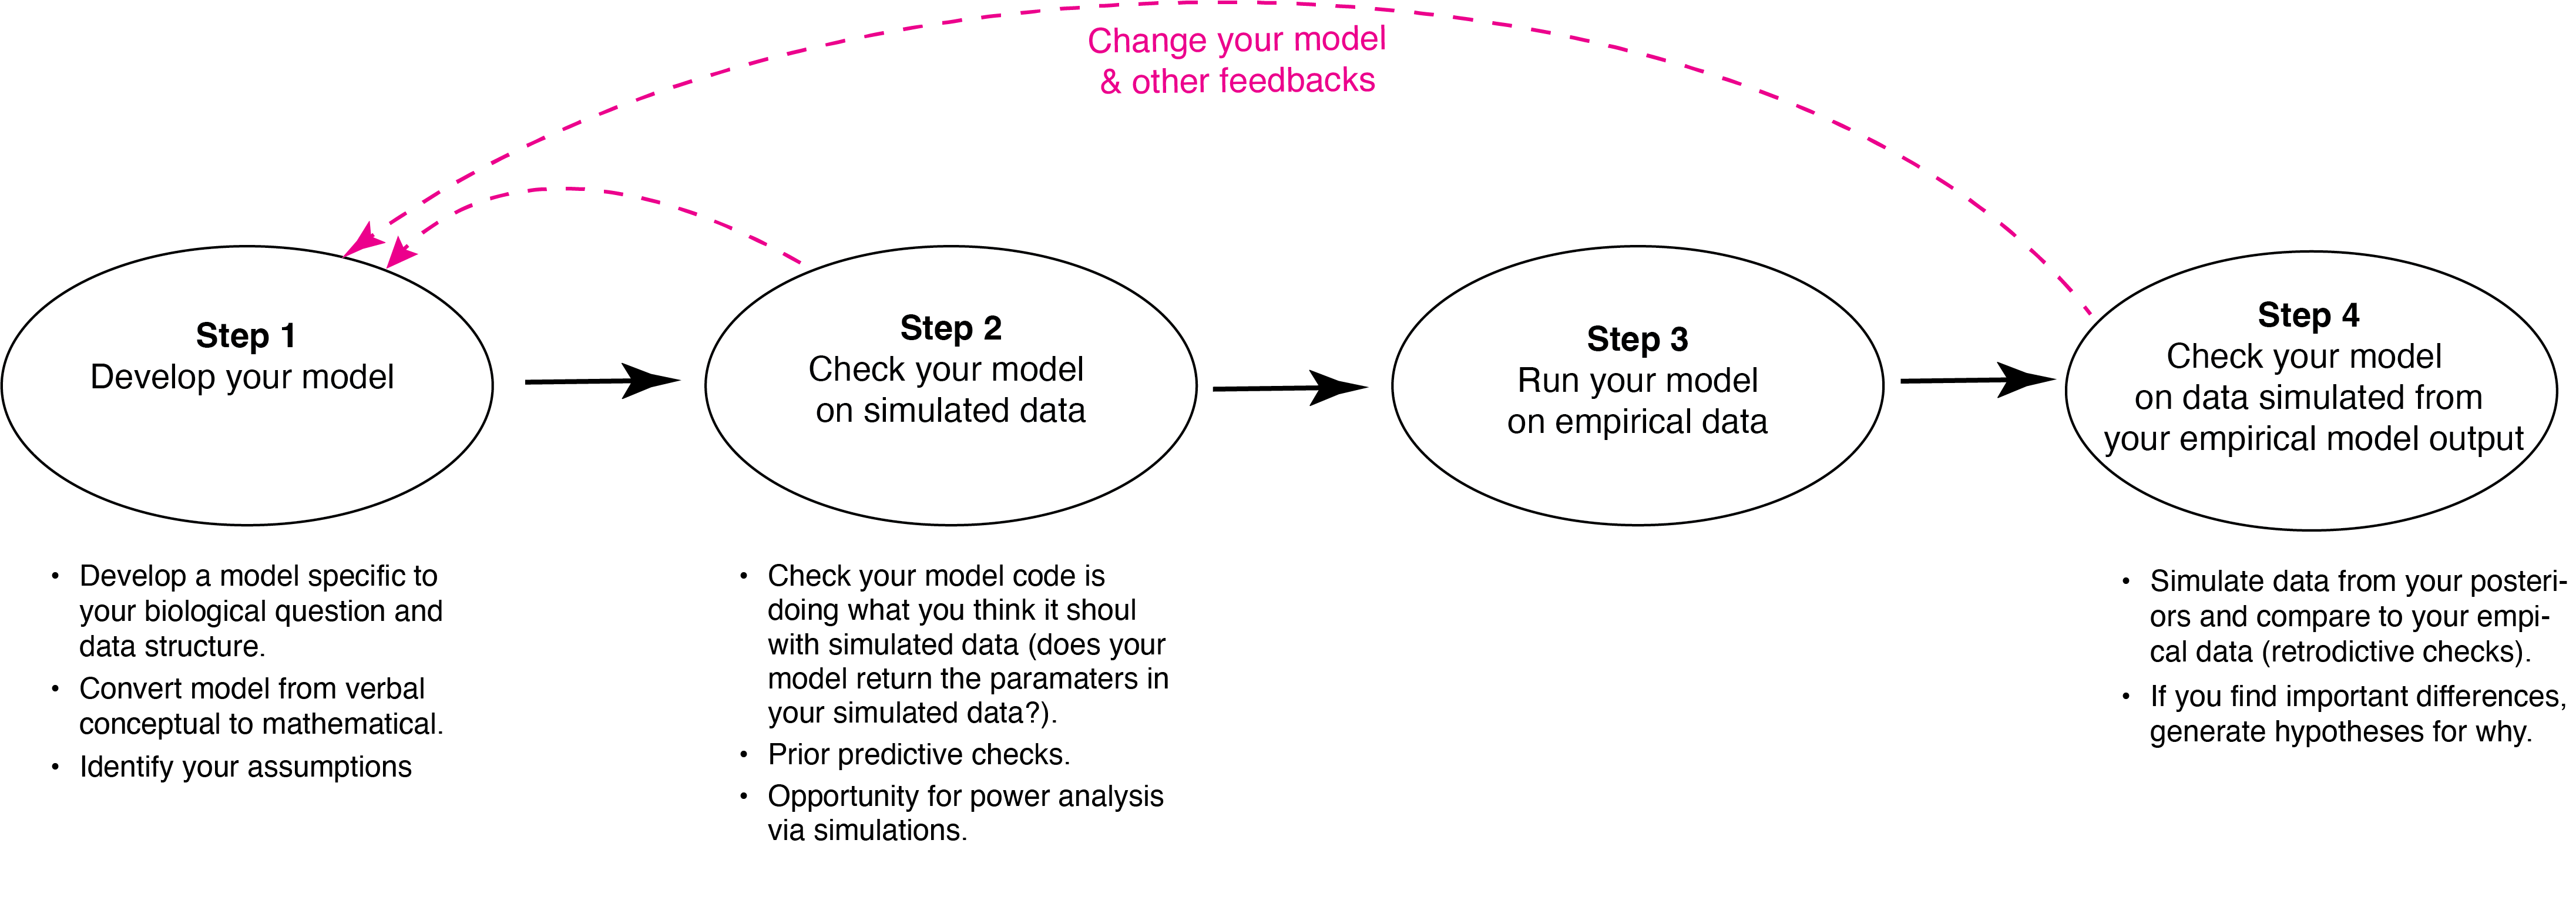
\includegraphics[width=1\textwidth]{figures/workflow.png}
\caption{A very basic workflow for Bayesian model fitting includes four major steps with potential feedbacks (pink dashed arrows) and begins with testing your model through simulated (test) data.}
\label{fig:workflow}
\end{figure}

\begin{figure}[ht]
\centering
\noindent 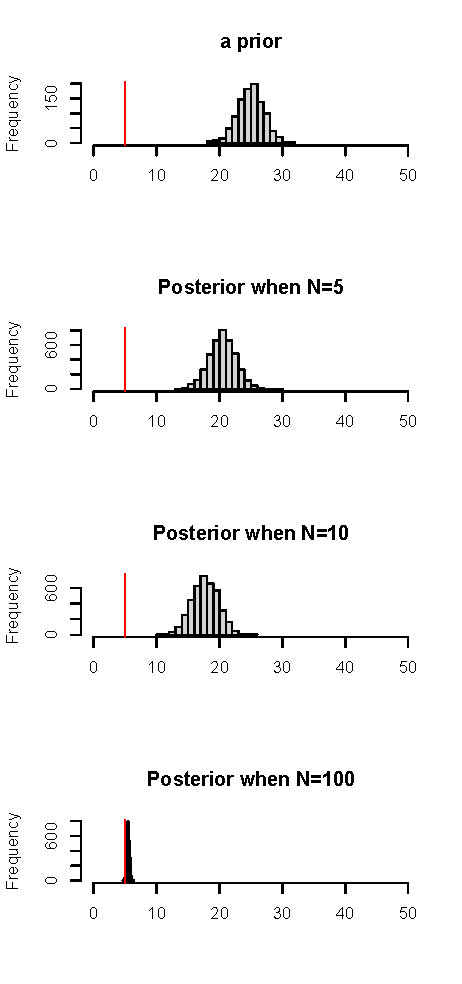
\includegraphics[width=0.5\textwidth]{examples/misspecifiedmodel/priorpostforflows.pdf}
\caption{A simple example of how we can use simulated data to understand calibration issues in a simple mis-specified model example. Here we know the true model underlying the data is $y=\alpha + \text{normal}(0, \sigma)$ where $\alpha$ is 5 (shown as red vertical line) and $\sigma$ is 2. The model, however, is mis-specified by a prior for $\alpha$ of $\text{normal}(25, 2)$ (in our experience, it is quite rare to have a prior informed by ecological knowledge be so far off, but this is an example). How mis-calibrated the model will be depends on the data: we show examples with a sample size ($N$) of 5, 10 and 100. }
\label{fig:misspecifyprior}
\end{figure}

\begin{figure}[ht]
\centering
\noindent 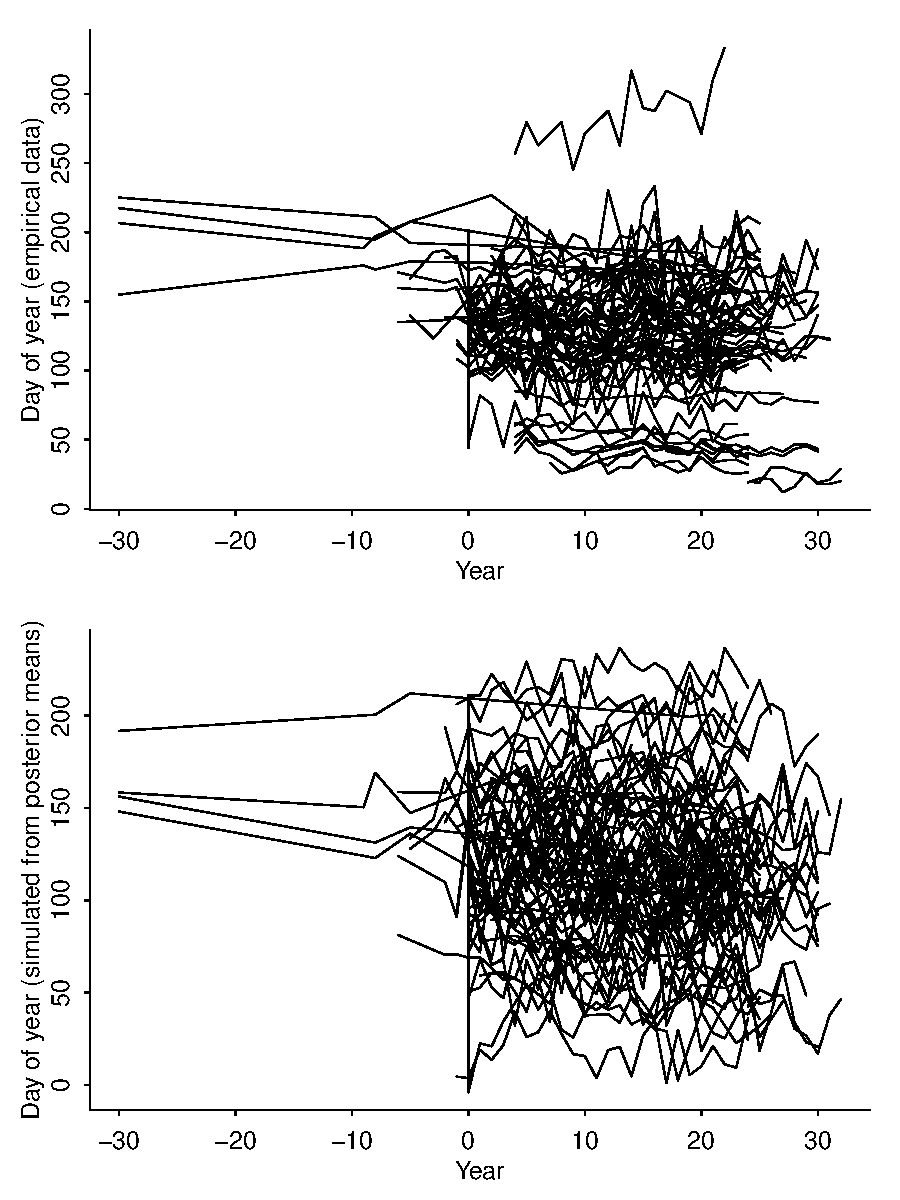
\includegraphics[width=0.6\textwidth]{examples/synchrony/graphs/rawvsonepredictivecheck.pdf}
\caption{Example of a single retrodictive check from time-series data of phenological events over time. The raw data (top) looks similar to one simulated dataset (bottom), based on existing species number, their respective $x$ data, and simulating from the parameters for each species. More predictive checks based on repeated simulations from the posterior, however, suggested issues in the model (see Fig. \ref{fig:retrodictivecheckSD}). See `An example workflow' in the Supplement for more details.}
\label{fig:retrodictivecheck}
\end{figure}


\begin{figure}[ht]
\centering
\noindent 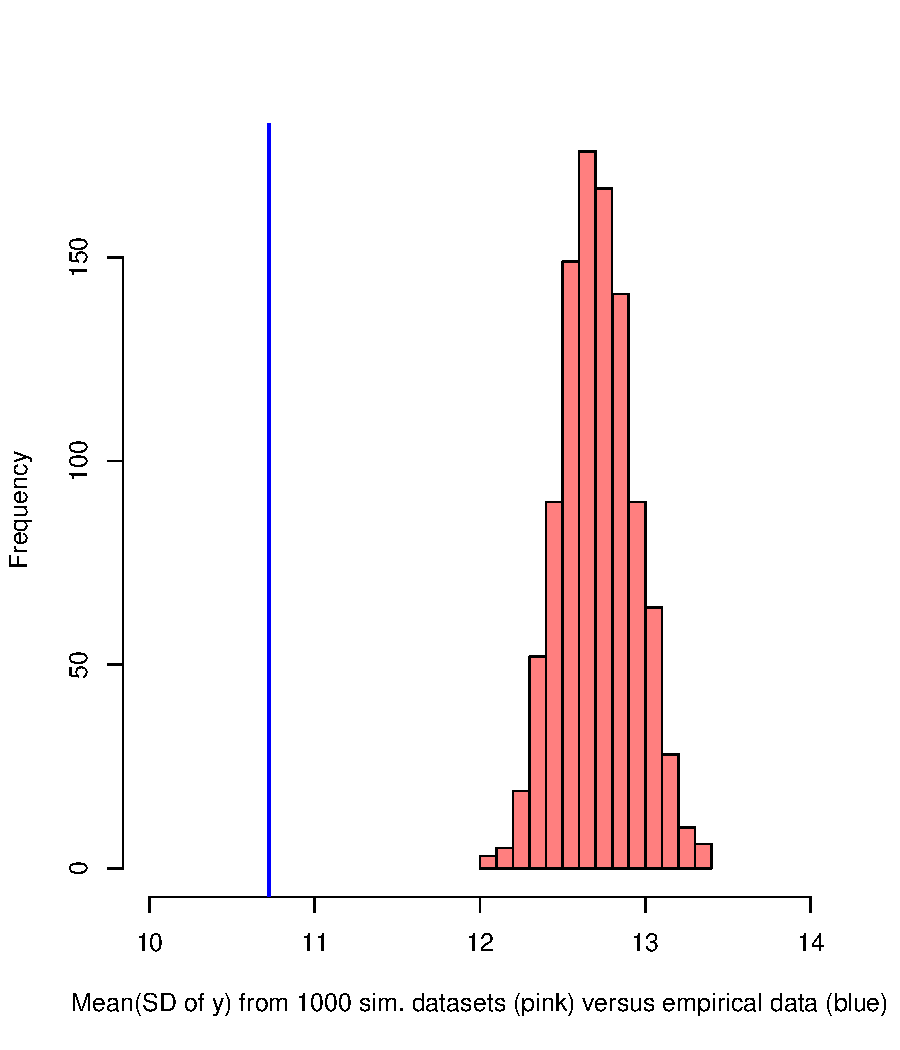
\includegraphics[width=0.5\textwidth]{examples/synchrony/graphs/retroSDsync.pdf}
\caption{Example of a retrodictive check, averaging across 1000 simulations (pink histogram), for a model of time-series data of phenological events over time, showed the model consistently over-predicted variance compared to the empirical data (blue line SD). See `An example workflow' in the Supplement for more details.}
\label{fig:retrodictivecheckSD}
\end{figure}

\end{document}


%%% Local Variables:
%%% mode: latex
%%% TeX-master: t
%%% End:
